\hypertarget{jay-leno}{%
\section{Jay Leno}\label{jay-leno}}

\begin{figure}[!ht]
  \begin{adjustwidth}{-\oddsidemargin-1in}{-\rightmargin}
    \centering
    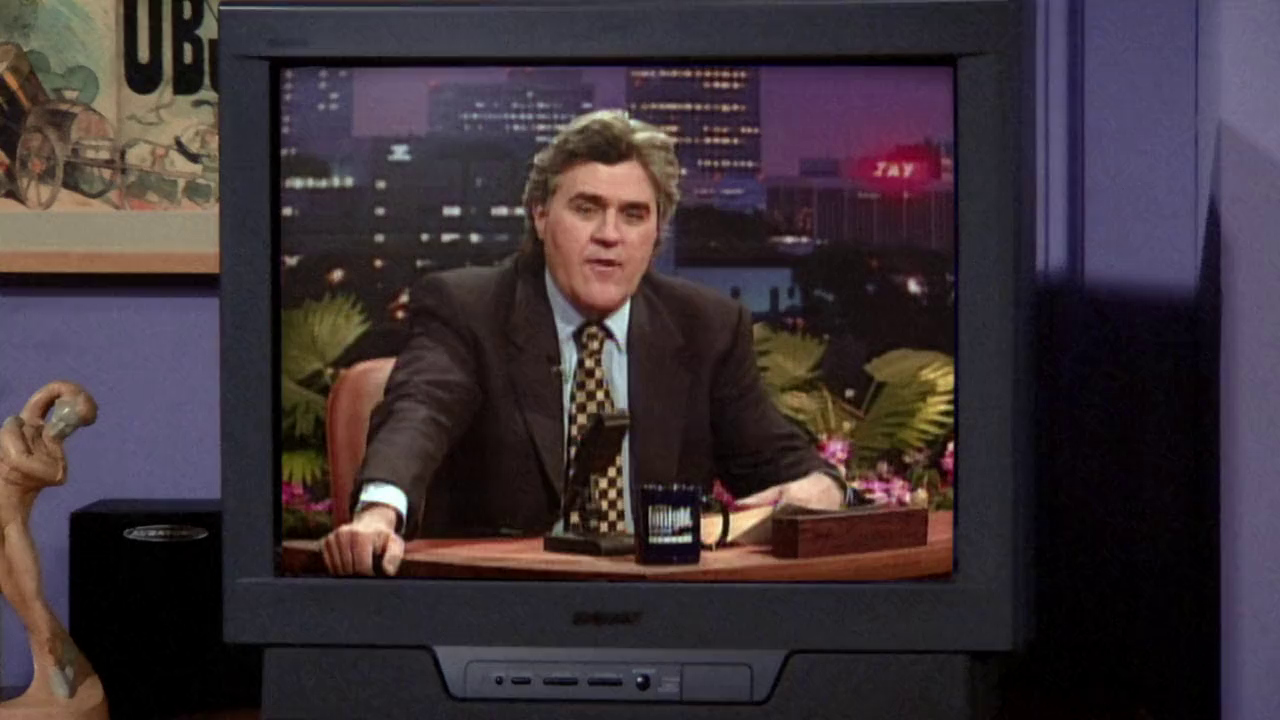
\includegraphics[trim={0 7cm 0 1cm,}, clip, width=\paperwidth]{./S01/img/11/jay-leno.png}
    \caption{Jay Leno\label{fig:jay-leno}}
  \end{adjustwidth}
\end{figure}

Os amigos assistem a escritora Nora Bing, mãe de Chandler, no programa
\emph{Tonight with Jay Leno} (1992-2014) do apresentador \emph{Jay
Leno}. O \emph{talk show} era filmado na California, no mesmo bloco do
estúdio da NBC onde era gravado \emph{Friends}.

O elenco de \emph{Friends} ainda faria uma reunião em 6 de Maio de 2004,
data em que os dois últimos episódios da série foram ao ar, num programa
especial apresentado no \emph{Central Perk}.

\begin{figure}
  \centering
  \begin{tikzpicture}
    \node [inner sep=0pt] at (0,0) {
      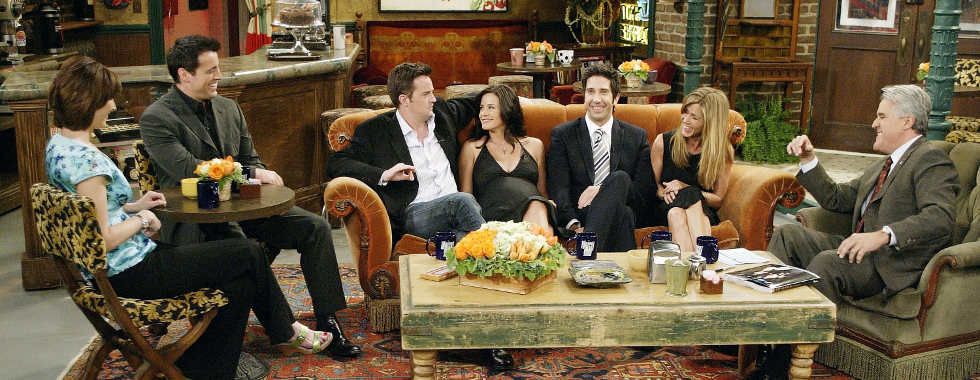
\includegraphics[width=0.8\textwidth,keepaspectratio]{./S01/img/11/jay-leno-friends-cast.jpg}
    };
    \draw [white, rounded corners=\ClipSep, line width=\ClipSep]
    (current bounding box.north west) --
    (current bounding box.north east) --
    (current bounding box.south east) --
    (current bounding box.south west) -- cycle
    ;
    \end{tikzpicture}
    \caption{Tonight with Jay Leno com elenco de Friends\label{fig:tonight-with-jay-leno-com-elenco-de-friends}}
\end{figure}

\hypertarget{referuxeancias}{%
\subsection{Referências}\label{referuxeancias}}

\begin{itemize}
\tightlist
\item
  \sloppy Página do ep. no Fandom Wiki (Inglês). \url{https://friends.fandom.com/wiki/The_One_With_Mrs._Bing}
\item
  \sloppy Wikipédia. \url{https://en.wikipedia.org/wiki/List_of_The_Tonight_Show_with_Jay_Leno_episodes_(2000%E2%80%932009)#May_5}
\item
  \sloppy The Last One, Part 1 - Fandom Wiki (Inglês). \url{https://friends.fandom.com/wiki/The_Last_One,_Part_1}
\end{itemize}

\hypertarget{weekend-at-bernies}{%
\section{Weekend at Bernie's}\label{weekend-at-bernies}}

\begin{figure}[!ht]
  \begin{adjustwidth}{-\oddsidemargin-1in}{-\rightmargin}
    \centering
    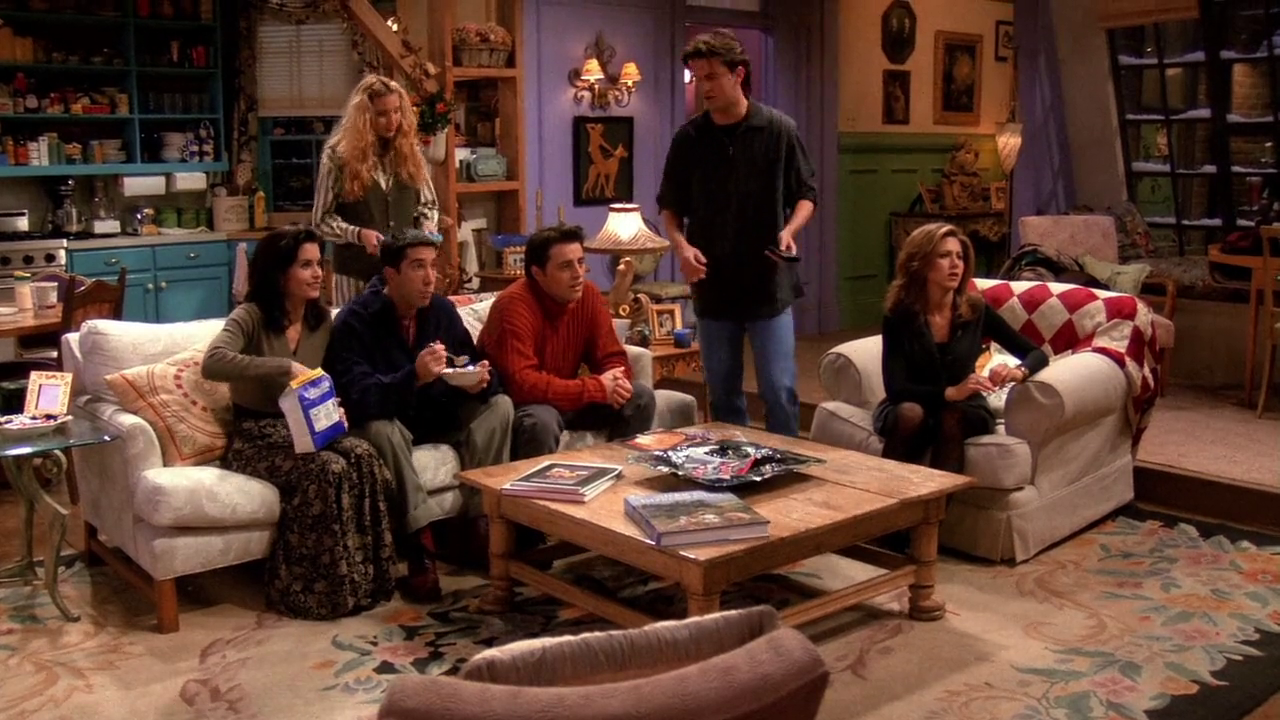
\includegraphics[trim={0 9cm 0 1cm,}, clip, width=\paperwidth]{./S01/img/11/weekend-at-bernies.png}
    \caption{Weekend at Bernie’s\label{fig:weekend-at-bernie-s}}
  \end{adjustwidth}
\end{figure}

\begin{tcolorbox}[enhanced,center upper,
    drop fuzzy shadow southeast, boxrule=0.3pt,
    lower separated=false,
    colframe=black!30!dialogoBorder,colback=white]
\begin{minipage}[c]{0.16\linewidth}
  \raisebox{\dimexpr-\height+\ht\strutbox\relax}{
    \centering 
\includegraphics[width=1.4cm]{./assets/img/chandler.png}
  }
   & \centering \scriptsize{Chandler}
\end{minipage}
\hfill
\begin{minipage}[c]{0.8\linewidth}
  \textbf{- Don't watch this. Weekend at Bernie's is on Showtime and HBO and Cinemax.}\\
  - Não vamos ver isto. Tá passando Um Morto Muito Louco na Showtime, HBO e Cinemax.
\end{minipage}
\end{tcolorbox}

Para evitar que os amigos vejam sua mãe falar sobre o novo livro dela,
Chandler sugere que eles assistam o filme \emph{Weekend at Bernie's}
(1989). O filme também é citado no episódio
\textbf{\textcolor{primarycolor}{S04E12 - Aquele com os embriões}} como
sendo o favorito da Rachel.

Chandler ainda cita \emph{Showtime}, \emph{HBO} e \emph{Cinemax}, todas
redes de televisão por assinatura americanas.

\begin{figure}
  \centering
  \begin{tikzpicture}
    \node [inner sep=0pt] at (0,0) {
      
\includegraphics[width=0.8\textwidth,keepaspectratio]{./S01/img/11/weekend-at-bernies-poster.jpg}
    };
    \draw [white, rounded corners=\ClipSep, line width=\ClipSep]
    (current bounding box.north west) --
    (current bounding box.north east) --
    (current bounding box.south east) --
    (current bounding box.south west) -- cycle
    ;
    \end{tikzpicture}
    \caption{Weekend at Bernie’s - Poster\label{fig:weekend-at-bernie-s-poster}}
\end{figure}

\hypertarget{referuxeancias-1}{%
\subsection{Referências}\label{referuxeancias-1}}

\begin{itemize}
\tightlist
\item
  \sloppy IMDB. \url{https://www.imdb.com/title/tt0098627/}
\item
  \sloppy Página do ep. no Fandom Wiki (Inglês). \url{https://friends.fandom.com/wiki/The_One_With_Mrs._Bing}
\item
  \sloppy Página do quiz (S04E12) no Fandom Wiki (Inglês). \url{https://friends.fandom.com/wiki/The_Contest}
\end{itemize}

\hypertarget{les-mystuxe8res-de-new-york}{%
\section{Les Mystères de New York}\label{les-mystuxe8res-de-new-york}}

\begin{figure}[!ht]
  \begin{adjustwidth}{-\oddsidemargin-1in}{-\rightmargin}
    \centering
    
\includegraphics[trim={0 8cm 0 1cm,}, clip, width=\paperwidth]{./S01/img/11/les-mysteres-de-new-york.png}
    \caption{Les Mystères de New York\label{fig:les-myst-res-de-new-york}}
  \end{adjustwidth}
\end{figure}

No apartamento de Chandler e Joey é possível ver um poster de \emph{Les
Mystères de New York} (1915), versão francesa do seriado estadunidense
\emph{The Exploits of Elaine}. Baseado na obra de \emph{Arthur B. Reeve}
(1880-1936), conta a história do detetive e cientista \emph{Craig
Kennedy}, que usa seus aparelhos de laboratório para descobrir a
identidade do assassino de \emph{Elaine Dodge}, que ficou conhecido como
\emph{A mão do diabo}.

Essa versão do seriado foi concebida pelo escritor \emph{Pierre
Decourcelle} (1856-1926). O poster é uma campanha promocional entre o
filme e o jornal francês \emph{Le Matin}, já que \emph{Decourcelle}
estava publicando uma versão impressa da história.

\begin{figure}
  \centering
  \begin{tikzpicture}
    \node [inner sep=0pt] at (0,0) {
      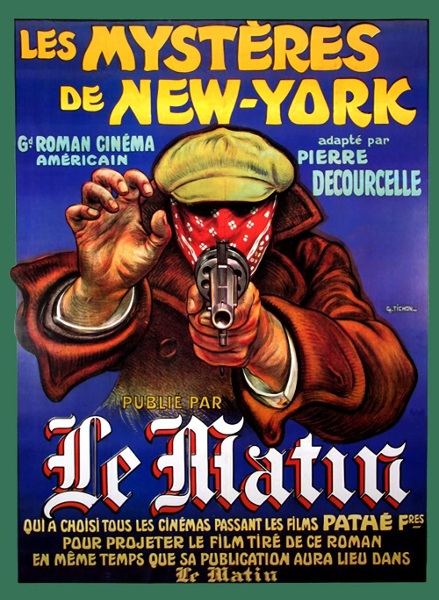
\includegraphics[width=0.4\textwidth,keepaspectratio]{./S01/img/11/les-mysteres-de-new-york-poster.jpg}
    };
    \draw [white, rounded corners=\ClipSep, line width=\ClipSep]
    (current bounding box.north west) --
    (current bounding box.north east) --
    (current bounding box.south east) --
    (current bounding box.south west) -- cycle
    ;
    \end{tikzpicture}
    \caption{Les Mystères de New York - Poster\label{fig:les-myst-res-de-new-york-poster}}
\end{figure}

\hypertarget{referuxeancias-2}{%
\subsection{Referências}\label{referuxeancias-2}}

\begin{itemize}
\tightlist
\item
  \sloppy The One with the Illustrated Posters (Inglês). \url{https://illustrationchronicles.com/The-One-with-the-Illustrated-Posters}
\item
  \sloppy Serial Squadron (Inglês). \url{http://serialsquadron.com/sites/ithacamademovies/serials/elaine/}
\item
  \sloppy IMDB. \url{https://www.imdb.com/title/tt0003897/}
\item
  \sloppy Wikipédia. \url{https://pt.wikipedia.org/wiki/The_Exploits_of_Elaine}
\item
  \sloppy Mucem (Francês). \url{https://www.mucem.org/programme/les-mysteres-de-new-york-exploits-elaine}
\end{itemize}

\hypertarget{ux43aux435ux43dux433ux443ux440ux443--ux431ux43eux43aux441ux435ux440-kangaroo-boxer}{%
\section{Кенгуру -Боксер (Kangaroo
Boxer)}\label{ux43aux435ux43dux433ux443ux440ux443--ux431ux43eux43aux441ux435ux440-kangaroo-boxer}}

\begin{figure}[!ht]
  \begin{adjustwidth}{-\oddsidemargin-1in}{-\rightmargin}
    \centering
    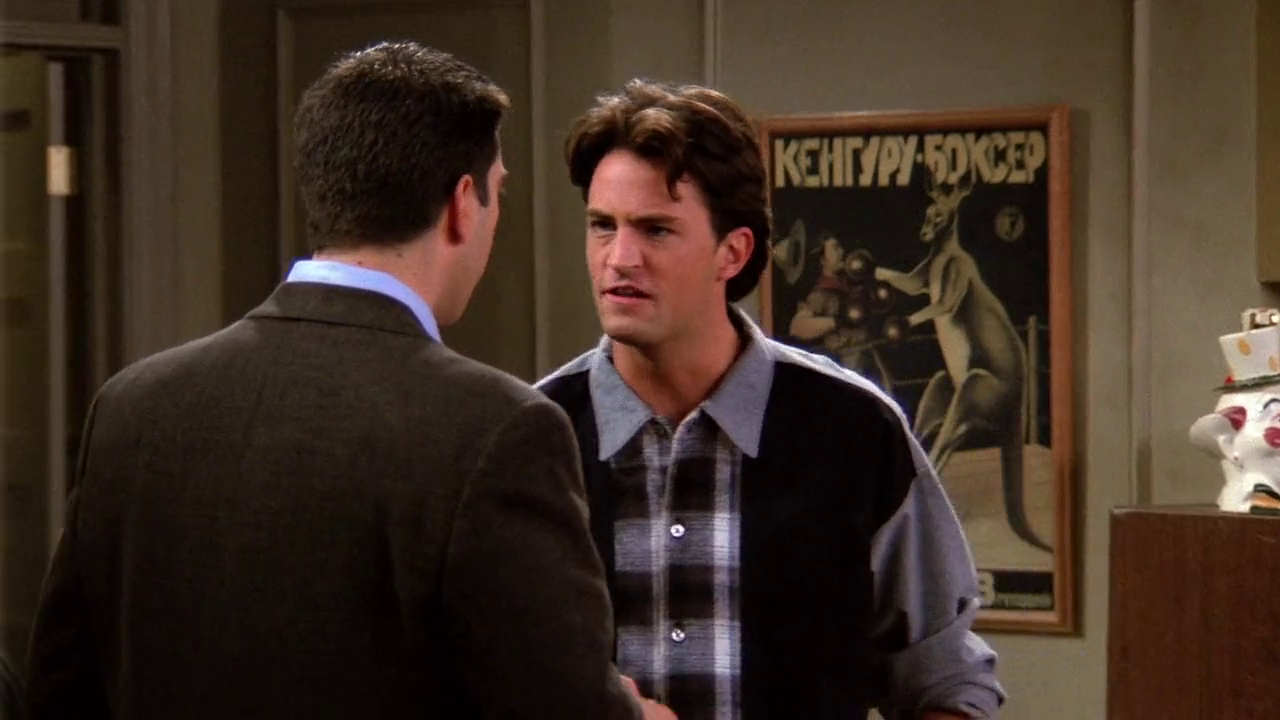
\includegraphics[trim={0 7cm 0 1cm,}, clip, width=\paperwidth]{./S01/img/11/kangaroo-boxer.png}
    \caption{Kangaroo Boxer\label{fig:kangaroo-boxer}}
  \end{adjustwidth}
\end{figure}

Ainda no apartamento dos rapazes, na parede oposta, podemos ver o poster
\emph{Кенгуру -Боксер (Kangaroo Boxer)}, que é uma referência à família
circense \emph{Durov} (1912), responsável por trazer renome e prestígio
ao circo Russo. São conhecidos por serem ótimos palhaços e treinadores
de animais.

\begin{figure}
  \centering
  \begin{tikzpicture}
    \node [inner sep=0pt] at (0,0) {
      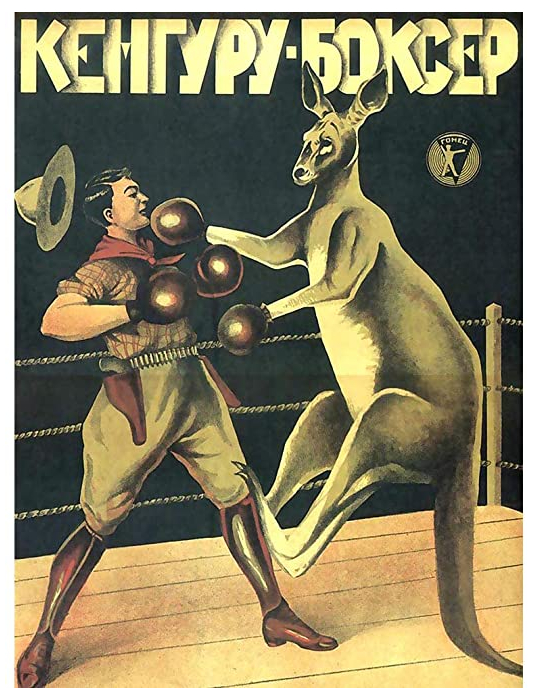
\includegraphics[width=0.4\textwidth,keepaspectratio]{./S01/img/11/kangaroo-boxer-poster.jpg}
    };
    \draw [white, rounded corners=\ClipSep, line width=\ClipSep]
    (current bounding box.north west) --
    (current bounding box.north east) --
    (current bounding box.south east) --
    (current bounding box.south west) -- cycle
    ;
    \end{tikzpicture}
    \caption{Kangaroo Boxer - Poster\label{fig:kangaroo-boxer-poster}}
\end{figure}

Não foi possível encontrar referências diretas de uma luta entre
\emph{Durov} e um canguru, mas o poster destaca a habilidade da família
no treinamento de animais dos mais variados, inclusive um hipopótamo. Um
fato importante foi a criação de um novo método de treinamento, o qual
não envolvia maus-tratos aos animais.

\begin{figure}
  \centering
  \begin{tikzpicture}
    \node [inner sep=0pt] at (0,0) {
      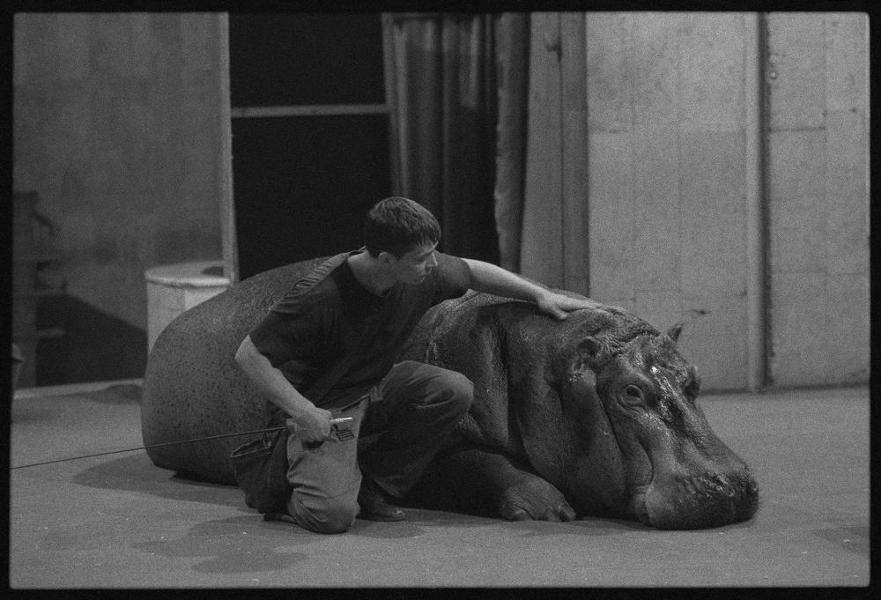
\includegraphics[width=0.6\textwidth,keepaspectratio]{./S01/img/11/durov-hipopotamo.jpg}
    };
    \draw [white, rounded corners=\ClipSep, line width=\ClipSep]
    (current bounding box.north west) --
    (current bounding box.north east) --
    (current bounding box.south east) --
    (current bounding box.south west) -- cycle
    ;
    \end{tikzpicture}
    \caption{Durov - Hipopótamo\label{fig:durov-hipop-tamo}}
\end{figure}

\hypertarget{referuxeancias-3}{%
\subsection{Referências}\label{referuxeancias-3}}

\begin{itemize}
\tightlist
\item
  \sloppy The One with the Illustrated Posters (Inglês). \url{https://illustrationchronicles.com/The-One-with-the-Illustrated-Posters}
\item
  \sloppy Website oficial (Russo). \url{https://www.ugolokdurova.ru/istoriya-teatra}
\item
  \sloppy Circopedia (Inglês). \url{http://www.circopedia.org/The_Durov_Dynasty}
\end{itemize}
